\documentclass[10pt]{article}
\usepackage{blindtext}
\usepackage{graphicx}
\usepackage{multirow}
\usepackage{amsmath}

\newtheorem{problem}{Problem}

\begin{document}

\title{Efficient Selection of Optimal Time Points Over Biological Time-Series Data}
\date{}

\maketitle

\section{Methods}

In this paper, we propose an efficient framework to identify subset of time points
jointly over gene expression time-series data for multiple genes. Our
proposed solution is different than the existing sampling based approaches since
the existing methods focus mostly on selecting subset of important time
points only over single gene. In addition, several other methods are
based on active learning which is not always valid for biological gene
expression data due to the nature of the experiments. For instance, multiple genes can be sampled simultaneously
once the time point is fixed which may not be modeled perfectly by
active learning based approaches. In general, our proposed solution is important since:
%
\begin{itemize}
\item There is still a space for improvement to identify subset of
  important time points since previous solutions are all based on heuristics. For
  instance,~\cite{bar2012} samples gene expression values at uniformly
  distributed time points which is not guaranteed to be the optimal. 
\vspace{0.05cm}
\item Efficient methods can greatly decrease experiment cost without
  trading off accuracy of the expression values. 
\end{itemize}
%
More formally, let $G$ be the set of genes which expression we are interested in
measuring/predicting, and $T = \{t_{1}, t_{2}, \ldots, t_{T}\}$ be the
set of all sampled time points. We assume that experiments is repeated
$D$ times; expression of each gene over each time points is mesured
$D$ times. In these experiments, let $e_{gt}^{d}$ be the expression value for gene $g \in G$, $t \in T$ across $d$'th repeat of
the experiment. We define $D_{g} = \{e_{gt}^{d}\,,\, t \in T, d \in 1,\ldots,D\}$ as the data for gene $g$ over all
replicates and time points $T$.

We assume that we have a predefined budget $k$ which is the
maximum number of time points we can sample~(we simply
assume that sampling each time point has same cost). We are interested
in selecting $k$ number of time points which minimizes the prediction error
of the rest of the unselected time points where we predict
expression values of unsampled time points by smoothing splines. In
our problem, $t_{1}$ and $t_{T}$ define the first and end points, so
they will always be a part of solution. It can be defined
formally as in Problem~\ref{prob:prob1}:
%
\begin{problem}\label{prob:prob1}
Given $D_{g}$ for genes $g \in G$, and number of points $k$ to select,
we are interested in identifying the subset of $k-2$ time points among
$T \setminus \{t_{1}, t_{T}\}$ which minimizes the prediction error of the expression values of remaining time points by
smoothing splines.
\end{problem}

\subsection{The Algorithm}

Here, we propose the following iterative solution to tackle
Problem~\ref{prob:prob1}. Initially, we select $k-2$ number of time
points~($t_{1}$ and $t_{T}$ are already in the solution) by one of the
heuristics that are defined in detail in Section~\ref{sec:init}. Then,
we keep adding one point among the remaining points 
and remove one point until there is no improvement in the error
of the remaining time points. In each iteration, we select the
point pair with the minimum error among all $(k-2)(T-k)$ point
pairs as our solution, and keep iterating until there is no
improvement. Figure~\ref{fig:algo} summarizes the iterative approach. 

\begin{figure}
\centering
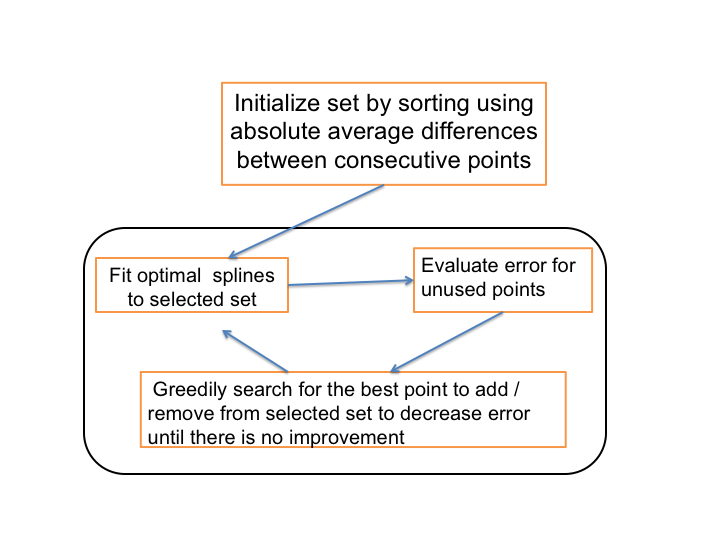
\includegraphics[scale=0.4]{algo.png}
\caption{Summary of our Method}
\label{fig:algo}
\end{figure}

\subsection{Initial Point Selection}\label{sec:init}

Initial selection of $k$ points has a significant effect on the results. We found
uniform partition and absolute value difference heuristics to perform
the best.

Uniform partition heuristic partitions the set of all time points $T$
into $k-1$ intervals of almost equal size by dynamic programming. Then, it uses $k$ interval
boundaries including $t_{1}$ and $t_{T}$ as initial solution. On the other hand, we absolute value
difference heuristic to perform better than uniform partition
heuristic. In this case, we sort all points except $t_{1}$ and $t_{T}$ by average absolute
difference with respect to the neighbouring time points as in:
%
\begin{equation}
m_{t_{i}} = \frac{\sum_{g \in G} \sum_{d \in D}\,|e_{g t_{i-1}}^{d} - e_{g t_{i+1}}^{d}|}{2 \sum_{g \in G} |D_{g}|}
\end{equation}
%
where then it selects the top $k-2$ points with maximum $m_{t_{i}}$ as
initial solution. 
%We have also experimented with xxx heuristic which did not perform better than the heuristics above.

\subsection{Iterative Step}\label{sec:iterative}

Iterative step exhaustively takes out each single
point from the existing solution and adds a point from the remaining
points into the solution. Let $C$ be the current solution of time points, and $C^{*}$ be the best solution
identified by iterative step. We are interested in finding a point
pair $(t_{a}, t_{d}$) among $(k-2)(T-k)$ point pairs which minimizes the following error for new
solution $C^{*} = C \setminus \{t_{d}\} \cup \{t_{a}\}$:
%
\begin{equation}
\textit{error}_{C^{*}} = \frac{\sum_{g \in G} \sum_{d \in D}\, \sum_{t \in
    T \setminus C^{*}}|\hat{e}_{gt} - e_{gt}^{d}|}{\sum_{g \in G}
  \sum_{d \in D} \sum_{t \in
    T \setminus C^{*}} 1}
\end{equation}
%
where $\hat{e}_{gt}$ is our estimate of the expression of gene $g$ at
time $t$ by fitting a smoothing spline. This iterative step continues until there is
no improvement in the error of the remaining time points. 

\section{Results}

\bibliographystyle{plain} 
\bibliography{expressbib}


\end{document}